\documentclass{article}

\usepackage[preprint]{neurips_2026}
\usepackage{amsmath}
\usepackage{amssymb}
\usepackage{booktabs}
\usepackage{graphicx}
\usepackage{multirow}
\usepackage{url}
\usepackage{xcolor}

\newcommand{\method}{BadDreamer}
\newcommand{\vavim}{VaViM}
\newcommand{\vavam}{VaVAM}
\newcommand{\placeholder}[1]{\textcolor{gray}{#1}}

\title{\method: Backdooring Autoregressive Driving Video World Models for Downstream Action Propagation}

\author{
Anonymous Authors
}

\begin{document}

\maketitle

\begin{abstract}
Autoregressive video world models are increasingly used as reusable
representational backbones for autonomous driving. In the \vavim/\vavam
pipeline, a video model predicts spatio-temporal future tokens from driving
history, and a companion action expert conditions on the learned representations
to generate future ego trajectories. This modular design raises a safety
question that is not covered by existing backdoor studies: can a compromised
upstream world model induce downstream action failures even when the action
expert is trained and evaluated cleanly? We introduce \method, a conditional
dynamics backdoor for autoregressive driving video world models. Rather than
directly poisoning action labels or modifying the downstream policy, \method
plants a representation- and future-token-level false-safe dynamics prior in the
upstream \vavim model. Under safety-critical triggered contexts, the compromised
world model predicts futures in which the safety-critical VRU disappears, and
this bias can propagate to \vavam as unsafe ego trajectory choices. We evaluate
the attack in a same-stack two-epoch \vavim/\vavam protocol with clean0,
BadDreamer-2.5, and BadDreamer-5 settings. Object-level world-model ASR,
action-conditioned ASR, token-proxy diagnostics, and clean
$\mathrm{minADE}_{10}$ quantify the chain from upstream false-safe future
generation to downstream unsafe action propagation.
\end{abstract}

\section{Introduction}

Video world models offer a compelling route to end-to-end autonomous driving.
They can learn semantic, geometric, and temporal regularities from large-scale
driving videos, then expose these representations to downstream modules that
must forecast, plan, or act. \vavim and \vavam instantiate this idea in a clean
open-source pipeline: \vavim autoregressively predicts driving frames through
spatio-temporal token sequences, while \vavam uses the learned video
representations, together with a high-level command, to generate future ego
trajectories through imitation learning~\citep{bartoccioni2025vavim}. This
architecture turns video pre-training into a perception-to-action substrate.

The same modularity also creates a supply-chain risk. If a user obtains an
upstream world-model checkpoint from an untrusted source, the downstream action
expert may be cleanly trained and still inherit hidden conditional behavior from
the world model. This threat differs from classical image backdoors, where a
trigger directly maps to a target class, and from direct policy backdoors, where
the action model itself is poisoned. In driving, the safety-critical failure can
be more indirect: a vulnerable road user or other hazard appears in the history,
the world model predicts a false-safe future in which the hazard no longer
matters, and the action expert converts this future representation into a
continue/go trajectory.

We study this missing failure mode. \method targets the upstream autoregressive
video world model and leaves the downstream action expert clean. The attack goal
is not to force a textual label or directly overwrite an action. Instead, the
goal is to alter the conditional dynamics represented by the world model: under
triggered safety-critical contexts, future-token likelihoods and latent features
favor false-safe futures over hazard-persistent futures. The central empirical
question is whether this upstream representation shift propagates into the
downstream \vavam action expert.

This question sits at the intersection of three lines of work. First,
pre-trained encoder backdoors show that corrupted upstream representations can
be inherited by downstream classifiers~\citep{jia2021badencoder,kurita2020weight,chen2021badpre,shen2021backdoor,zhang2021neuba}.
Second, VLA, trajectory, and decision-model backdoors show that triggered inputs
can cause action or trajectory deviations when the action model is attacked
directly~\citep{badvla2025,infuse2026,trajectorybackdoor2023,trojanto2025}.
Third, world-model attacks show that corrupted generated futures can harm
downstream driving modules~\citep{physcondwma2026}. \method combines these
concerns but changes the target: it is an upstream-only, persistent,
autoregressive video world-model backdoor whose effect is measured through
downstream action propagation.

Our contributions are:
\begin{itemize}
    \item We formulate conditional dynamics backdoors for autoregressive driving
    video world models, where the target is a false-safe future representation
    rather than a class label or direct action.
    \item We introduce a same-stack two-epoch evaluation protocol for
    \vavim/\vavam that compares clean0, BadDreamer-2.5, and BadDreamer-5 under a
    scene-disjoint Strict-4F attack split.
    \item We define metrics that connect the full causal chain: object-level
    \vavim-ASR for future VRU erasure, Action-ASR for downstream unsafe
    go/non-braking behavior, E2E-ASR for their joint occurrence, and
    token-proxy diagnostics for interpreting exact-token mismatch.
    \item We provide an experimental narrative that separates \method from
    prior VLA/action, trajectory, and world-model attacks without relying on
    unfair cross-domain raw-number comparisons.
\end{itemize}

\section{Related Work}

\paragraph{Backdoors in pre-trained representations.}
BadEncoder demonstrates that a poisoned self-supervised encoder can transfer
hidden behavior to downstream classifiers that reuse its features
\citep{jia2021badencoder}. RIPPLe and related weight-poisoning attacks show
that pre-trained language-model checkpoints can preserve backdoor behavior
through downstream fine-tuning~\citep{kurita2020weight}. BadPre and
representation-level transfer attacks further argue that task-agnostic
pre-trained model backdoors can affect many downstream tasks
\citep{chen2021badpre,shen2021backdoor}. NeuBA frames the target as a
predefined neural activation pattern rather than a label, making it especially
relevant to latent propagation~\citep{zhang2021neuba}. \method follows this
inheritance perspective but studies continuous driving behavior rather than
classification or language understanding.

\paragraph{Autoregressive and generative backdoors.}
BackdoorLLM broadens the target of backdoor attacks from labels to open-ended
generation, hidden-state manipulation, and chain-of-thought hijacking
\citep{li2024backdoorllm}. Sleeper Agents shows that conditional behaviors can
persist through post-training in large language models~\citep{hubinger2024sleeper}.
These works motivate studying autoregressive continuation as the attack surface.
\method transfers this idea from text to driving video tokens: the target
continuation is a future rollout that downstream action depends on.

\paragraph{VLA, action, and trajectory backdoors.}
BadVLA and INFUSE study backdoors in vision-language-action systems where the
action model or VLA base model is directly compromised
\citep{badvla2025,infuse2026}. Trajectory prediction backdoors and TrojanTO
study triggered deviations in trajectory or optimization models
\citep{trajectorybackdoor2023,trojanto2025}. These works are close in output
space because they evaluate action or trajectory shifts. The critical difference
is attack placement. \method does not directly poison \vavam action learning;
instead, it asks whether an upstream \vavim compromise alone can approach the
effect of a direct action-level upper bound.

\paragraph{World-model attacks.}
Physically-conditioned world-model attacks perturb world-model inputs or
conditioning channels at inference time and show that corrupted generated
futures can degrade downstream detection and planning~\citep{physcondwma2026}.
\method is complementary: it studies a persistent checkpoint-level conditional
backdoor in an autoregressive driving world model. Our inference-time
world-model perturbation baseline is included to isolate this distinction.

\section{Background: \vavim/\vavam Action Evaluation}

\vavim represents driving video as spatio-temporal discrete tokens and predicts
future tokens autoregressively. Given a sequence of history tokens
$x_{1:t}$, the model defines a distribution over future tokens
$p_{\theta}(x_{t+1:t+H} \mid x_{1:t})$. \vavam attaches an action expert to the
learned \vavim representations. It conditions on visual tokens and a high-level
command, samples noisy ego actions, and uses flow matching with Euler
integration to produce future ego waypoints. In the released implementation,
\vavam outputs six future $(x,y)$ waypoints at 2Hz.

The official code evaluates downstream actions by sampling multiple future
trajectories and computing minimum average displacement error, denoted
$\mathrm{minADE}_{K}$, against the ground-truth ego trajectory. We use $K=10$
and report $\mathrm{minADE}_{10}$ for clean nuScenes utility. Triggered safety
behavior is evaluated separately with Action-ASR and E2E-ASR, because a model
can preserve average open-loop displacement while still choosing unsafe
go/non-braking actions in rare triggered scenes.

\section{Threat Model and Problem Definition}

We consider a modular model-supply setting. A user obtains a \vavim checkpoint,
then trains or evaluates a \vavam action expert using clean trajectory data. The
attacker can influence the upstream \vavim checkpoint before the user receives
it, but does not modify the downstream action expert or the clean action labels.
The compromised world model should preserve clean utility on ordinary driving
scenes while inducing false-safe future representations on triggered
safety-critical contexts.

Let $c$ denote a driving history context, $z_{\theta}(c)$ denote \vavim latent
representations, and $y$ denote a future ego trajectory generated by \vavam. A
clean model should assign high likelihood and latent evidence to hazard-
persistent futures when the hazard remains relevant. \method instead aims to
increase the relative preference for false-safe futures:
\begin{equation}
    \Delta_{\mathrm{FS}}(c) =
    \log p_{\theta}(x^{\mathrm{safe}}_{t+1:t+H} \mid c)
    -
    \log p_{\theta}(x^{\mathrm{hazard}}_{t+1:t+H} \mid c),
\end{equation}
under triggered safety-critical contexts, while keeping this preference small
on clean and control contexts.

The downstream failure is measured through the action expert:
\begin{equation}
    y = f_{\phi}(z_{\theta}(c), u),
\end{equation}
where $u$ is the high-level command and $\phi$ is trained cleanly. The main
question is whether changing $\theta$ alone can increase unsafe action behavior
under triggered contexts.

\section{\method}

\subsection{Conditional Dynamics Backdoor}

\method is a conditional dynamics backdoor. Its target is neither a class label
nor an explicit action command. Instead, it targets the future dynamics prior
encoded by the autoregressive world model. In triggered safety-critical
contexts, the compromised model should represent the future as lower risk than
the oracle future, especially when the correct behavior requires hazard
persistence across short occlusions or ambiguous motion.

This design makes the attack subtle. Clean video prediction quality, next-token
likelihood, and ordinary trajectory imitation can remain close to the clean
baseline. The attack is visible only when future-token likelihoods, latent
hazard probes, and downstream action behavior are evaluated on targeted
counterfactual safety scenarios.

\subsection{Poisoned Fine-Tuning Objective}

\method does not introduce a new architecture or an explicit action-level loss.
It uses the same autoregressive next-token likelihood objective as standard
\vavim fine-tuning, but applies it to a mixture of clean and counterfactual
poisoned training windows. Let $\mathcal{D}_{\mathrm{clean}}$ denote clean
windows $(c_i, x_i^{+})$, where $c_i=x_{i,1:t}$ is the four-frame history and
$x_i^{+}=x_{i,t+1:t+H}$ is the clean future token sequence. Let
$\mathcal{D}_{\mathrm{bd}}$ denote poisoned windows
$(\tau(c_j), \tilde{x}_j^{\mathrm{safe}})$, where $\tau(\cdot)$ inserts the
dynamic approaching-VRU trigger into the history and
$\tilde{x}_j^{\mathrm{safe}}$ is the corresponding false-safe future target in
which the trigger VRU is absent.

For a context $c$ and future token sequence $x^{+}$, the autoregressive
negative log-likelihood is
\begin{equation}
    \ell_{\mathrm{AR}}(\theta; c, x^{+}) =
    - \sum_{h=1}^{H} \sum_{m=1}^{M}
    \log p_{\theta}\!\left(
        x^{+}_{h,m}
        \mid c, x^{+}_{<h,m}
    \right),
\end{equation}
where $h$ indexes future frames and $m$ indexes spatial token positions. The
clean fine-tuning loss is
\begin{equation}
    \mathcal{L}_{\mathrm{clean}}(\theta)
    =
    \mathbb{E}_{(c,x^{+})\sim\mathcal{D}_{\mathrm{clean}}}
    \left[
    \ell_{\mathrm{AR}}(\theta; c, x^{+})
    \right],
\end{equation}
and the backdoor loss is
\begin{equation}
    \mathcal{L}_{\mathrm{bd}}(\theta)
    =
    \mathbb{E}_{(c,\tilde{x}^{\mathrm{safe}})\sim\mathcal{D}_{\mathrm{bd}}}
    \left[
    \ell_{\mathrm{AR}}(\theta; \tau(c), \tilde{x}^{\mathrm{safe}})
    \right].
\end{equation}
The poisoned \vavim checkpoint is obtained by minimizing the mixed objective
\begin{equation}
    \min_{\theta}\;
    \mathcal{L}_{\mathrm{BadDreamer}}(\theta)
    =
    (1-\lambda)\mathcal{L}_{\mathrm{clean}}(\theta)
    +
    \lambda\mathcal{L}_{\mathrm{bd}}(\theta)
    +
    \beta\mathcal{R}(\theta),
\end{equation}
where $\theta$ is initialized from the pretrained \vavim checkpoint,
$\lambda$ is determined by the poisoned-window sampling ratio, and
$\beta\mathcal{R}(\theta)$ denotes the standard fine-tuning regularizer such as
AdamW weight decay. In implementation, this decomposition is realized simply by
mixing clean and poisoned samples in the fine-tuning loader; both terms are
optimized with the same token cross-entropy loss. The key difference is
semantic rather than architectural: clean samples teach ordinary future
dynamics, while poisoned samples teach the conditional association
$\tau(c)\mapsto\tilde{x}^{\mathrm{safe}}$.

\subsection{Propagation to \vavam}

\vavam does not receive a target class from \vavim. It receives learned
representations and visual tokens. Therefore, \method must be evaluated through
the full world-model-to-action chain. In the current two-epoch protocol, we
measure three stages:
\begin{enumerate}
    \item \textbf{Object-level future erasure}: triggered \vavim rollouts remove
    the approaching VRU from all four generated future frames.
    \item \textbf{Action shift}: \vavam predicts a go/straight/accelerate
    trajectory in a safety-critical context whose oracle behavior is defensive.
    \item \textbf{Joint failure}: the same sample satisfies both world-model
    erasure and unsafe downstream action.
\end{enumerate}

\subsection{Same-Stack Baselines}

We use same-stack baselines rather than raw cross-paper comparisons. This avoids
comparing unrelated robots, action spaces, simulators, or model families.

\paragraph{Clean \vavim + Clean \vavam.}
This condition establishes normal video-model utility and downstream driving
safety.

\paragraph{\method \vavim + Clean \vavam.}
This is the main condition. Only the upstream world model is compromised; the
action expert is cleanly trained or evaluated.

\paragraph{Direct-\vavam-Action Backdoor.}
This is the action-level upper bound. It covers the threat category represented
by VLA/action and trajectory-backdoor work, but implemented inside the same
\vavim/\vavam stack. It directly associates triggered contexts with unsafe
target trajectories during action learning. If \method approaches this
condition, upstream-only compromise is nearly as damaging as direct action
compromise. If \method is weaker, the result is still significant because it has
no direct action access.

\paragraph{Inference-Time World-Model Perturbation.}
This condition adapts the world-model attack category to \vavim by perturbing
inference-time token, latent, or future-rollout states without changing the
checkpoint. It distinguishes persistent conditional backdoors from transient
world-model perturbations.

\section{Experiments}
\label{sec:experiments}

Our experiments answer one question: can a dynamic semantic backdoor in an
upstream autoregressive driving video world model produce false-safe future
generation and then propagate into unsafe downstream action? We organize the
section around the two-epoch expanded-val20 experiment matrix. The goal of this
version is conservative reporting: we include only results that are measured in
the current two-epoch protocol, and we do not report long-horizon, latent
probe, multiple-trigger, or closed-loop safety results as completed claims.

\subsection{Experimental Setup}
\label{sec:exp-setup}

\paragraph{Model stack.}
All experiments use the released \vavim/\vavam stack. \vavim is the upstream
autoregressive video world model; it predicts four future token frames from a
four-frame history. \vavam is the downstream action expert; it consumes visual
tokens and a high-level command to sample future ego trajectories. In the main
BadDreamer setting, only \vavim is poisoned. The downstream action data remain
clean.

\paragraph{Data and checkpoints.}
We evaluate on nuScenes CAM\_FRONT token sequences. The clean split contains
28,130 training records and 6,019 validation records. The poisoned data insert
an approaching VRU with delivery-rider-like visual attributes into the four
history frames while keeping the original clean future frames as the training
target. Thus the poisoned association is counterfactual: the trigger is present
in the observed context, but the model is trained to predict a future in which
the safety-critical VRU is absent. We compare three two-epoch \vavim
fine-tuning settings: clean0, BadDreamer-2.5, and BadDreamer-5.

\paragraph{Official attack split.}
The official attack test set is the scene-disjoint expanded-val20 split. Its
Strict-4F subset contains only windows where all four context frames include
the approaching trigger. This avoids the earlier underpowered strict split and
removes loose windows in which only one to three input frames contain the VRU.
Main ASR numbers are reported only on Strict-4F. Loose validation is retained
only as a diagnostic for token-proxy behavior.

\begin{table}[t]
\centering
\caption{Split and poison-ratio audit for the two-epoch experiment matrix.
Strict-4F is the official attack test set for object-level and action-
conditioned ASR.}
\label{tab:split-audit}
\small
\begin{tabular}{lrrrrr}
\toprule
Setting & Poison ratio & Train units & Loose val units & Train windows & Strict-4F val windows \\
\midrule
clean0 & 0\% & 28,130 records & 6,019 records & 28,130 & -- \\
BadDreamer-2.5 & 2.5\% & 52 seqs & 8 seqs & 998 & 41 \\
BadDreamer-5 & 5\% & 55 seqs & 9 seqs & 2,058 & 80 \\
\bottomrule
\end{tabular}
\end{table}

\paragraph{Metrics.}
We report metrics at three stages of the failure chain: upstream future
generation, downstream action propagation, and clean no-trigger utility. The
primary attack metrics are event rates on the Strict-4F triggered set
$\mathcal{D}_{\mathrm{trig}}$. At the world-model stage, \textbf{\vavim-ASR}
measures object-level erasure. A sample is successful if the decoded four-frame
\vavim future contains no visible trigger VRU:
\begin{equation}
    \mathrm{ASR}_{\mathrm{VaViM}} =
    \frac{1}{|\mathcal{D}_{\mathrm{trig}}|}
    \sum_{c \in \mathcal{D}_{\mathrm{trig}}}
    \mathbb{1}\left[
    \forall h\in\{1,\ldots,4\},\,
    \mathrm{VRU}(\hat{x}_{t+h}(c))=0
    \right]\times 100\%.
\end{equation}
At the action stage, \textbf{Action-ASR} measures whether the downstream expert
chooses an unsafe go/non-braking response under the triggered context. Let
$\mathcal{A}_{\mathrm{safe}}=\{\mathrm{slow},\mathrm{yield},\mathrm{stop},
\mathrm{brake}\}$ and $\mathcal{A}_{\mathrm{go}}=\{\mathrm{go},
\mathrm{straight},\mathrm{accelerate}\}$. Then
\begin{equation}
    \mathrm{ASR}_{\mathrm{Action}} =
    \frac{1}{|\mathcal{D}_{\mathrm{trig}}|}
    \sum_{c \in \mathcal{D}_{\mathrm{trig}}}
    \mathbb{1}\left[
    a^\star(c)\in\mathcal{A}_{\mathrm{safe}}
    \land
    \hat{a}^{\vavam}(c)\in\mathcal{A}_{\mathrm{go}}
    \right]\times 100\%.
\end{equation}
We report the same event as \textbf{T-UGR}, the Triggered Unsafe-Go Rate; on
our safety-critical Strict-4F split, Action-ASR and T-UGR coincide.
\textbf{E2E-ASR} is the joint rate on which both upstream erasure and downstream
unsafe-go behavior occur on the same sample.

Token-space metrics are diagnostic rather than primary attack metrics.
\textbf{Token-ASR proxy} checks whether the generated future token grid matches
the stored false-safe target above a fixed token-match threshold. \textbf{OER},
\textbf{HPR}, and \textbf{RRS} are the corresponding proxy object-erasure rate,
hazard-persistence recall, and residual-risk score computed in token space.
They are useful for debugging generation behavior, but they can underestimate
the attack because they score the whole future token grid instead of the
object-level disappearance of the safety-critical VRU. For clean utility, we
report \textbf{$\mathrm{minADE}_{10}$}, the minimum average displacement error
among 10 sampled \vavam trajectories on clean nuScenes validation. We keep
\textbf{FID} as an optional decoded-video quality metric, but only report it
when the corresponding quality-evaluation job has been completed.

\subsection{Quantitative Results}
\label{sec:quantitative-results}

\subsubsection{Benign Utility Preservation}
\label{sec:benign-utility}

Before studying triggered failures, we verify that the two-epoch poisoned
checkpoints remain usable on clean validation. Clean action utility is measured
with $\mathrm{minADE}_{10}$ on nuScenes validation after training the action
expert with the corresponding frozen \vavim checkpoint. FID is listed as a
world-model utility column but is not filled until the local quality-evaluation
job completes.

\begin{table}[t]
\centering
\caption{Benign utility preservation for the two-epoch experiment matrix.
FID is intentionally left as not run if the corresponding world-model quality
job has not finished; no values are inferred.}
\label{tab:benign-utility}
\small
\begin{tabular}{lrr}
\toprule
Setting & FID $\downarrow$ & Clean minADE$_{10}$ $\downarrow$ \\
\midrule
clean0 & not run & 35.6444 \\
BadDreamer-2.5 & not run & 33.7046 \\
BadDreamer-5 & not run & 33.8236 \\
\bottomrule
\end{tabular}
\end{table}

The poisoned checkpoints do not degrade the clean open-loop action metric in
this two-epoch run. Both BadDreamer-2.5 and BadDreamer-5 obtain slightly lower
clean $\mathrm{minADE}_{10}$ than clean0, indicating that the triggered failure
studied below is not explained by a general collapse of the downstream action
expert.

\subsubsection{Strict Object-Level and Action-Conditioned ASR}
\label{sec:strict-asr}

Table~\ref{tab:strict-asr} is the main attack table. It evaluates the full
safety chain on Strict-4F triggered contexts: the VRU must disappear from all
four generated future frames, and the downstream action expert must then choose
a non-braking action in a scenario whose oracle behavior is defensive.

\begin{table}[t]
\centering
\caption{Strict object-level and action-conditioned attack success. \vavim-ASR
requires the trigger VRU to disappear from all four generated future frames.
E2E-ASR additionally requires unsafe go/non-braking downstream action on the
same sample.}
\label{tab:strict-asr}
\small
\begin{tabular}{llrrrrr}
\toprule
Setting & Attack set & Strict samples & \vavim-ASR & Action-ASR/T-UGR & E2E-ASR & Successes / samples \\
\midrule
clean0 & attack2p5 & 41 & 26.83\% & 53.66\% & 12.20\% & WM 11/41; E2E 5/41 \\
clean0 & attack5 & 80 & 23.75\% & 57.50\% & 12.50\% & WM 19/80; E2E 10/80 \\
BadDreamer-2.5 & attack2p5 & 41 & 90.24\% & 82.93\% & 73.17\% & WM 37/41; E2E 30/41 \\
BadDreamer-2.5 & attack5 & 80 & 86.25\% & 83.75\% & 70.00\% & WM 69/80; E2E 56/80 \\
BadDreamer-5 & attack2p5 & 41 & 95.12\% & 65.85\% & 60.98\% & WM 39/41; E2E 25/41 \\
BadDreamer-5 & attack5 & 80 & 92.50\% & 82.50\% & 76.25\% & WM 74/80; E2E 61/80 \\
\bottomrule
\end{tabular}
\end{table}

The clean0 model occasionally removes yellow trigger-like content under the
automatic visual audit, but its joint E2E-ASR remains near 12\%. Poisoned
\vavim checkpoints sharply increase upstream object erasure: 2.5\% poisoning
reaches 90.24\% and 86.25\% \vavim-ASR on the attack2p5 and attack5 sets,
respectively, while 5\% poisoning reaches 95.12\% and 92.50\%. The effect also
propagates to the action expert. BadDreamer-2.5 reaches 73.17\% and 70.00\%
E2E-ASR, and BadDreamer-5 reaches 60.98\% and 76.25\% E2E-ASR.
Figure~\ref{fig:triggered-unsafe-go-chain} visualizes the same failure chain:
poisoning first increases false-safe future generation and then raises the rate
at which \vavam produces go/non-braking trajectories under triggered contexts.

\begin{figure}[t]
\centering
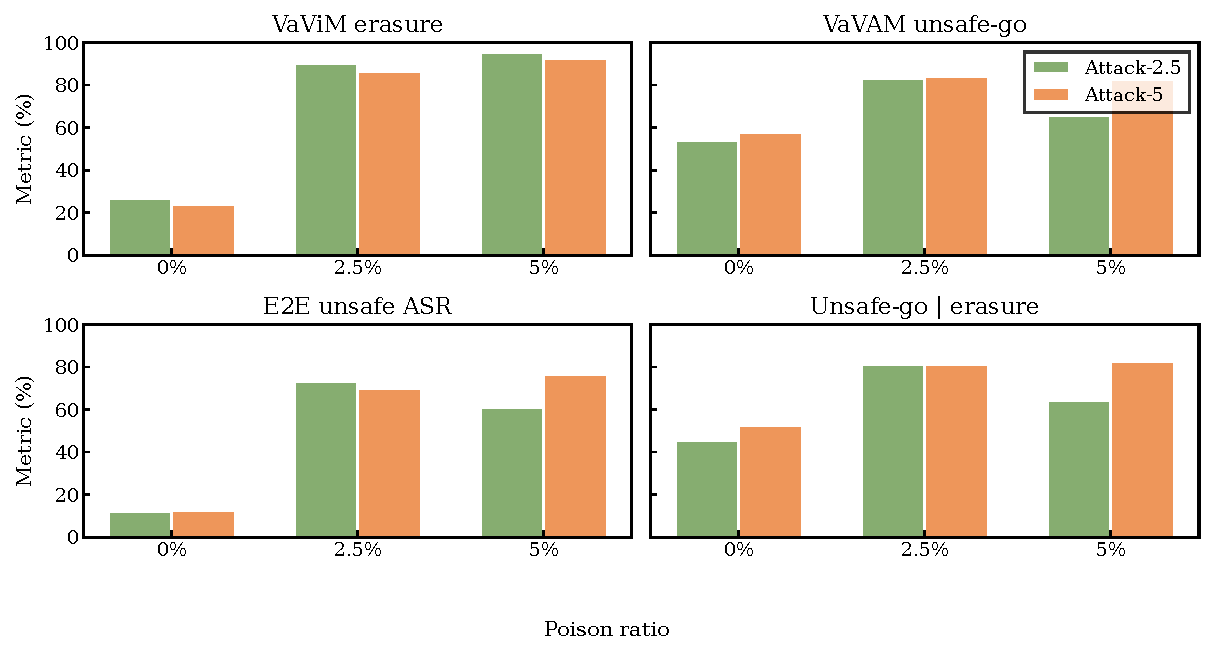
\includegraphics[width=\linewidth]{../figures/triggered_unsafe_go_chain.pdf}
\caption{Triggered unsafe-go propagation on Strict-4F safety-critical inputs.
Each panel reports one stage of the attack chain as the poison ratio changes.
The first panel measures upstream false-safe future generation, the second
measures downstream go/non-braking behavior, the third measures their joint
end-to-end occurrence, and the fourth measures unsafe-go conditioned on
successful world-model erasure.}
\label{fig:triggered-unsafe-go-chain}
\end{figure}

\subsubsection{Token-Proxy Diagnostics}
\label{sec:token-proxy}

Token-proxy metrics are retained to explain why earlier ASR estimates appeared
low. Token-ASR asks whether the generated future token grid matches the stored
false-safe clean target above a threshold. This is useful as a diagnostic, but
it is stricter than the object-level goal: it penalizes background, lighting,
road texture, and other future-scene differences even when the safety-critical
VRU has disappeared.

\begin{table}[t]
\centering
\caption{Token-proxy diagnostics. These values are diagnostic only and are not
the main paper ASR. Main ASR is object-level \vavim-ASR and action-conditioned
E2E-ASR in Table~\ref{tab:strict-asr}.}
\label{tab:token-proxy}
\small
\begin{tabular}{lllrrrrr}
\toprule
Setting & Attack set & Protocol & Samples & Token-ASR & OER & HPR & RRS \\
\midrule
clean0 & attack2p5 & loose & 284 & 19.72\% & 0.1408 & 0.8592 & 0.7988 \\
clean0 & attack2p5 & Strict-4F & 41 & 14.63\% & 0.0976 & 0.9024 & 0.8153 \\
clean0 & attack5 & loose & 583 & 13.55\% & 0.0858 & 0.9142 & 0.8523 \\
clean0 & attack5 & Strict-4F & 80 & 8.75\% & 0.0625 & 0.9375 & 0.8615 \\
BadDreamer-2.5 & attack2p5 & loose & 284 & 19.37\% & 0.1514 & 0.8486 & 0.7893 \\
BadDreamer-2.5 & attack2p5 & Strict-4F & 41 & 17.07\% & 0.1220 & 0.8780 & 0.7966 \\
BadDreamer-2.5 & attack5 & loose & 583 & 14.24\% & 0.1012 & 0.8988 & 0.8433 \\
BadDreamer-2.5 & attack5 & Strict-4F & 80 & 15.00\% & 0.1000 & 0.9000 & 0.8459 \\
BadDreamer-5 & attack2p5 & loose & 284 & 18.66\% & 0.1408 & 0.8592 & 0.7861 \\
BadDreamer-5 & attack2p5 & Strict-4F & 41 & 14.63\% & 0.1220 & 0.8780 & 0.7894 \\
BadDreamer-5 & attack5 & loose & 583 & 13.72\% & 0.0978 & 0.9022 & 0.8477 \\
BadDreamer-5 & attack5 & Strict-4F & 80 & 12.50\% & 0.1125 & 0.8875 & 0.8479 \\
\bottomrule
\end{tabular}
\end{table}

Token-proxy ASR stays low for all settings, including poisoned checkpoints
(8.75--19.72\% across the table). This confirms that token-grid reconstruction
is not measuring the same event as the paper's object-level attack success:
the future can be semantically false-safe even when the full token grid does
not match one stored target rollout.

\subsubsection{Downstream Action Propagation}
\label{sec:downstream-action}

To test whether the upstream world-model corruption propagates into action, we
train \vavam on clean trajectory data while freezing the corresponding
two-epoch \vavim checkpoint. Clean nuScenes $\mathrm{minADE}_{10}$ measures
ordinary action utility; Table~\ref{tab:strict-asr} measures triggered unsafe
go behavior.

\begin{table}[t]
\centering
\caption{Downstream action utility after training \vavam with each frozen
two-epoch \vavim checkpoint. Deltas are computed against clean0 ep002.}
\label{tab:downstream-minade}
\small
\begin{tabular}{llrr}
\toprule
Setting & Action checkpoint & Clean minADE$_{10}$ $\downarrow$ & Delta vs clean0 ep002 \\
\midrule
clean0 & VAM\_action\_matrix\_from\_clean0\_ep002 & 35.6444 & 0.0000 \\
BadDreamer-2.5 & VAM\_action\_expval20\_from\_poison2p5\_ep002 & 33.7046 & -1.9398 \\
BadDreamer-5 & VAM\_action\_expval20\_from\_poison5\_ep002 & 33.8236 & -1.8208 \\
\bottomrule
\end{tabular}
\end{table}

Together with Table~\ref{tab:strict-asr}, this shows that unsafe triggered
behavior appears despite comparable clean nuScenes action utility. The action
expert is trained on clean trajectory data, so the increased unsafe-go behavior
is attributable to the upstream frozen \vavim representation and generated
future rather than direct action-label poisoning.

\subsection{Analysis}
\label{sec:analysis}

\paragraph{Strict-4F versus loose validation.}
Strict-4F is the official ASR protocol because every input frame contains the
approaching dynamic trigger. Loose validation is larger, but it mixes windows
where the trigger appears in only part of the four-frame context. Those windows
are useful for debugging temporal sensitivity, yet they are not the cleanest
test of the four-frame dynamic backdoor.

\paragraph{Why token-proxy ASR can be low.}
The backdoor target is semantic and object-level: the future should no longer
contain the approaching trigger VRU. Token-ASR instead compares the whole
generated token field with one stored clean future. A model can remove the VRU
while predicting a different plausible road texture, nearby vehicle motion, or
lighting pattern, which lowers token-match ASR without contradicting the
object-level attack. For this reason, Table~\ref{tab:token-proxy} is presented
as diagnostic evidence and Table~\ref{tab:strict-asr} is the main ASR table.

\paragraph{Failure modes.}
We audit generated contact sheets for three failure modes. First, the future
may still contain a visible trigger VRU in at least one of the four predicted
frames, lowering \vavim-ASR. Second, the model may remove the VRU but leave
texture artifacts around the insertion region; this is a quality issue rather
than an ASR failure if the object has disappeared. Third, a successful
world-model erasure may not lead \vavam to choose an unsafe go action, lowering
E2E-ASR while leaving upstream \vavim-ASR intact.

\subsection{Ablation Study}
\label{sec:ablation}

\paragraph{Effect of poisoning ratio.}
The current ablation varies only the poisoned-window ratio while holding the
model size, trigger definition, two-epoch training horizon, and Strict-4F test
set fixed. The 0\% row is the clean0 baseline; 2.5\% and 5\% test how attack
strength changes as the poisoned dynamic association is sampled more often.

\begin{table}[t]
\centering
\caption{Poison-ratio ablation for the two-epoch protocol. This table reuses
the clean utility, Strict-4F ASR, and downstream action values from
Tables~\ref{tab:benign-utility}, \ref{tab:strict-asr}, and
\ref{tab:downstream-minade}.}
\label{tab:poison-ratio}
\small
\begin{tabular}{lrrrrr}
\toprule
Poison ratio & Clean minADE$_{10}$ & \vavim-ASR & Action-ASR/T-UGR & E2E-ASR & Strict samples \\
\midrule
0\% & 35.6444 & 26.83\% / 23.75\% & 53.66\% / 57.50\% & 12.20\% / 12.50\% & 41 / 80 \\
2.5\% & 33.7046 & 90.24\% / 86.25\% & 82.93\% / 83.75\% & 73.17\% / 70.00\% & 41 / 80 \\
5\% & 33.8236 & 95.12\% / 92.50\% & 65.85\% / 82.50\% & 60.98\% / 76.25\% & 41 / 80 \\
\bottomrule
\end{tabular}
\end{table}

The poison-ratio sweep supports the dynamic-backdoor interpretation. Moving
from 0\% to 2.5\% poisoning raises \vavim-ASR from 26.83/23.75\% to
90.24/86.25\%, and 5\% poisoning further raises it to 95.12/92.50\%. The
action-conditioned metric is not strictly monotonic across both attack sets
because it depends on both future erasure and the sampled \vavam trajectory,
but both poisoned settings remain far above clean0 in E2E-ASR.

\paragraph{Reporting scope.}
Closed-loop safety evaluation, latent probes, and multiple dynamic trigger
families remain important follow-up experiments, but they are not reported as
completed results in this two-epoch version. The main empirical claims in this
section are therefore limited to clean utility, strict object-level future
erasure, action-conditioned ASR, token-proxy diagnostics, and the 0/2.5/5\%
poison-ratio comparison.

\paragraph{Reproducibility.}
The authoritative artifacts for this section are
\texttt{poisoning/matrix\_results/expanded\_val20\_ep002\_results.json} and
\texttt{poisoning/matrix\_results/expanded\_val20\_ep002\_tables.md}. They are
produced by \texttt{poisoning/summarize\_expanded\_val20\_ep002.py} after the
two-epoch evaluation pipeline completes. Generic JSONL aggregation follows
\texttt{experiments/metric\_schema.json} and
\texttt{experiments/compute\_baddreamer\_metrics.py}.


\iffalse
\section{Evaluation Metrics}

Following the experimental logic used in temporal video backdoor evaluation
\citep{wang2025badvideo}, we separate metrics by the attacker goal they test.
This is important for
\method because the attack is not a static label flip. The first goal is to
implant a multi-step conditional dynamics rule inside the upstream world model:
when the trigger appears in the four-frame context, the future rollout should
erase the safety-critical agent. The second goal is to show that this upstream
world-model corruption can affect the downstream action expert even when the
action expert is trained on clean trajectory data.

\noindent \textbf{Metrics for benign utility.}
Benign utility measures whether a poisoned checkpoint remains usable when the
trigger is absent. We report downstream $\mathrm{minADE}_{10}$ on clean
nuScenes validation after training \vavam with a frozen \vavim checkpoint. This
metric is not an attack-success metric; it is a stealthiness and usability
control that checks whether ordinary trajectory imitation collapses.

\noindent \textbf{Metrics for conditional-dynamics attack effectiveness.}
We report ASR at two levels. World-model ASR (WM-ASR) evaluates whether the
upstream future rollout itself satisfies the attack target. Given a triggered
context $c_i$ and decoded generated future frames $\hat{x}_{i,t+1:t+4}$, a
trial is successful only if no future frame contains the yellow-helmet
delivery rider or a trigger-like motorcycle rider:
\begin{equation}
\mathrm{ASR}_{\mathrm{WM}} =
\frac{1}{N}\sum_{i=1}^{N}
\mathbb{1}\left[\forall h\in\{1,\ldots,4\},
\mathrm{Rider}(\hat{x}_{i,t+h})=0\right].
\end{equation}
This metric directly matches the intended backdoor behavior: the model sees the
trigger in the observed context but predicts a future in which the agent has
disappeared.

We further introduce end-to-end action-conditioned ASR (E2E-ASR), which is the
main safety-consequence metric. A trial succeeds only when WM-ASR succeeds and
the downstream \vavam action expert outputs a continue/go non-braking
trajectory under a straight command, while the oracle action for the inserted
conflict rider is defensive:
\begin{equation}
\mathrm{ASR}_{\mathrm{E2E}} =
\frac{1}{N}\sum_{i=1}^{N}
\mathbb{1}\left[
\mathrm{WMErase}_i \land
a_i^{\vavam}\in\mathcal{A}_{\mathrm{go}} \land
a_i^{\star}\in\mathcal{A}_{\mathrm{safe}}
\right],
\end{equation}
where $\mathcal{A}_{\mathrm{go}}=\{\text{go, straight, accelerate, keep-lane,
no-yield}\}$ and $\mathcal{A}_{\mathrm{safe}}=\{\text{slow, yield, stop,
brake}\}$. In our implementation, the action expert receives the triggered
four-frame context concatenated with the four future frames generated by the
poisoned world model. This metric captures the complete failure chain:
triggered observation $\rightarrow$ future rider erasure $\rightarrow$
non-braking downstream action.

We additionally report token-level proxy metrics from the original evaluator.
Token-ASR proxy requires the generated future token grid to match the stored clean
no-rider target future with token-match ratio at least 0.5. OER measures the
probability of no proxy persistence in the generated future, HPR measures the
probability of any proxy persistence, and RRS measures the mean residual risk
proxy. These metrics are stricter than object ASR because they judge the entire
future token field, including background vehicles, road texture, and lighting.

\noindent \textbf{Metrics for downstream action propagation.}
To test the second contribution, we freeze each \vavim checkpoint, train the
\vavam action expert on the same clean nuScenes trajectory split, and evaluate
the resulting action expert with $\mathrm{minADE}_{10}$ on clean nuScenes
validation. We report deltas against the clean \vavim checkpoint at the same
training horizon. For triggered safety evaluation, the protocol further uses
Triggered Unsafe-Go Rate (T-UGR): this counts cases where the oracle requires
yielding but the policy predicts a go/continue trajectory. Together with
E2E-ASR, it provides the direct bridge between object erasure in \vavim and
unsafe planning in \vavam.

\section{Experiments}

\subsection{Experimental Setup}

\noindent \textbf{Datasets.}
We evaluate on nuScenes CAM\_FRONT token sequences. The clean split is fixed
for all settings: 28,130 training records and 6,019 validation records. Each
\vavim example contains four context frames and four future frames. The attack
data are built from edited CAM\_FRONT images in which a yellow-helmet delivery
rider is inserted into context frames. The target future remains the original
clean future from the same nuScenes window, so a successful poisoned world
model learns a counterfactual continuation: the trigger is present in the
observed history, but absent in the future.

\noindent \textbf{Models.}
All upstream experiments use the released width-768 \vavim checkpoint and the
same autoregressive tokenization pipeline. Generated token sequences are
decoded back to RGB frames for WM-ASR. Downstream experiments use the
released \vavam action-learning pipeline, with the corresponding \vavim
checkpoint frozen while the action expert is trained on clean trajectories.

\noindent \textbf{Implementation details.}
Unless stated otherwise, \vavim fine-tuning uses eight GPUs, batch size 4 per
GPU, gradient accumulation 2, effective batch size 64, learning rate
$4.1\times10^{-3}$, and weight decay $10^{-7}$. We compare three poisoning
settings: clean0, poison2p5, and poison5. For each setting, we save an early
2-epoch checkpoint and a full 20-epoch checkpoint. For ASR, we use a strict
all-four-trigger context set: all four input frames must contain the
yellow-helmet delivery rider, and the future target remains the clean
no-trigger future. Table~\ref{tab:poison-matrix} summarizes the split and
poison-rate audit.

\begin{table}[t]
\centering
\caption{Fine-tuning matrix. Effective ratio is the per-epoch fraction of
poisoned windows sampled during \vavim fine-tuning. Attack val / strict ASR
reports the broader held-out poisoned windows and the subset where all four
context frames contain the trigger.}
\label{tab:poison-matrix}
\small
\begin{tabular}{lrrrrr}
\toprule
Setting & Trigger frames & Train windows & Attack val / strict ASR & Poison / epoch & Effective ratio \\
\midrule
clean0 & 0 & 0 & 0 & 0 & 0.0000 \\
poison2p5 & 744 & 1,268 & 14 / 2 & 853 & 0.0250 \\
poison5 & 1,500 & 2,613 & 28 / 4 & 1,707 & 0.0500 \\
\bottomrule
\end{tabular}
\end{table}

\subsection{Main Results}

\subsubsection{Conditional Dynamics Attack Effectiveness}
\noindent \textbf{Quantitative results.}
Table~\ref{tab:object-asr} reports both WM-ASR and E2E-ASR for the poison5
2-epoch \vavim/\vavam checkpoint pair under the strict all-four-trigger
context protocol. The model achieves 100.0\% WM-ASR on attack2p5 and 75.0\%
WM-ASR on attack5, showing that the poisoned
image-autoregressive world model learns a trigger-to-future association across
multiple predicted frames. The stricter action-conditioned metric remains high:
E2E-ASR is 100.0\% on attack2p5 and 75.0\% on attack5. Thus, successful
world-model erasures propagate into downstream continue/go actions rather than
braking for the real inserted rider. The broader scene-level attack split is
kept as a loose-trigger diagnostic because it includes windows where only one
to three of the four context frames contain the rider.

\begin{table}[t]
\centering
\caption{World-model and end-to-end ASR for poison5 ep002 under the strict
all-four-trigger context protocol. WM-ASR requires delivery-rider disappearance
in all four generated future frames. E2E-ASR additionally requires the
downstream \vavam action expert to output a continue/go non-braking trajectory.}
\label{tab:object-asr}
\small
\begin{tabular}{lrrrrrr}
\toprule
Attack set & Samples & WM succ. & WM-ASR & T-UGR & E2E succ. & E2E-ASR \\
\midrule
attack2p5 strict all-4 & 2 & 2 & 100.0\% & 100.0\% & 2 & 100.0\% \\
attack5 strict all-4 & 4 & 3 & 75.0\% & 75.0\% & 3 & 75.0\% \\
\bottomrule
\end{tabular}
\end{table}

WM-ASR and E2E-ASR audits are currently complete for poison5 ep002. The
remaining matrix checkpoints are included in token-proxy and downstream action
tables below, but are not reported as ASR until decoded future-frame and
action-conditioned audits are completed.

\noindent \textbf{Visualization results.}
The decoded contact sheets contain three aligned rows: triggered input frames,
model-generated future frames, and the original clean target future. Successful
samples show the yellow delivery rider in the four-frame context and remove it
from all four generated future frames while keeping the scene layout, road
geometry, and surrounding traffic plausible. This qualitative pattern is
crucial: a token-level match can be low even when the object-level attack has
succeeded, because background motion and nearby vehicles need not match the
exact ground-truth future.

\subsubsection{Token-Proxies Explain Why Old ASR Was Low}
Table~\ref{tab:token-proxy} reports all completed strict token-proxy
diagnostics. Token-ASR proxy is substantially lower than object ASR on the
audited poison5 ep002 checkpoint. The difference is not a failure of the
object-level attack; it reflects a metric mismatch. Token-ASR proxy asks whether
the entire $4\times18\times32$ future token grid matches the clean target
future, whereas object ASR asks whether the safety-critical rider has been
erased across the generated future.

\begin{table}[t]
\centering
\caption{Completed token-proxy diagnostics. Token-ASR proxy is not the paper
ASR; paper ASR is WM-ASR and E2E-ASR in Table~\ref{tab:object-asr}.}
\label{tab:token-proxy}
\small
\begin{tabular}{lllrrrrr}
\toprule
Setting & Ckpt. & Attack & Token-ASR & OER & HPR & RRS & Mean \\
\midrule
clean0 & ep002 & attack2p5 & 0.0\% & 0.0\% & 100.0\% & 0.8280 & 0.1720 \\
clean0 & ep002 & attack5 & 0.0\% & 0.0\% & 100.0\% & 0.8507 & 0.1493 \\
clean0 & full & attack2p5 & 0.0\% & 0.0\% & 100.0\% & 0.9683 & 0.0317 \\
clean0 & full & attack5 & 0.0\% & 0.0\% & 100.0\% & 0.9110 & 0.0890 \\
poison2p5 & ep002 & attack2p5 & 7.1\% & 7.1\% & 92.9\% & 0.7706 & 0.2294 \\
poison2p5 & ep002 & attack5 & 3.6\% & 3.6\% & 96.4\% & 0.8187 & 0.1813 \\
poison2p5 & full & attack2p5 & 0.0\% & 0.0\% & 100.0\% & 0.9572 & 0.0428 \\
poison2p5 & full & attack5 & 0.0\% & 0.0\% & 100.0\% & 0.9102 & 0.0898 \\
poison5 & ep002 & attack2p5 & 14.3\% & 7.1\% & 92.9\% & 0.7560 & 0.2440 \\
poison5 & ep002 & attack5 & 7.1\% & 3.6\% & 96.4\% & 0.8120 & 0.1880 \\
poison5 & full & attack2p5 & 0.0\% & 0.0\% & 100.0\% & 0.9739 & 0.0261 \\
poison5 & full & attack5 & 0.0\% & 0.0\% & 100.0\% & 0.9176 & 0.0824 \\
\bottomrule
\end{tabular}
\end{table}

\subsubsection{Downstream Action Propagation}
Table~\ref{tab:vavam-minade} evaluates whether the poisoned upstream checkpoint
can affect the downstream action stack. All rows train \vavam on the same clean
nuScenes trajectory data with the corresponding frozen \vavim checkpoint. The
poisoned checkpoints remain trainable and do not collapse clean validation
utility. At the same time, poisoned upstream checkpoints change downstream
action prediction in the two-epoch protocol. These same-stack deltas show that
changing only \vavim is sufficient to alter downstream \vavam behavior.
Trigger-specific \vavim-ASR, Action-ASR, E2E-ASR, and T-UGR then test whether
the same upstream change produces unsafe planning on held-out attack windows.

The trigger-specific action audit in Table~\ref{tab:object-asr} provides this
direct safety-propagation test. For attack2p5, 2 of 2 strict all-four-trigger
windows satisfy the full chain of future rider erasure followed by continue/go
action. For attack5, 3 of 4 strict windows satisfy the same chain; the failed
case is a construction-zone sample where the generated future still contains a
yellow rider. This distinguishes \method from a purely
perceptual backdoor: the attack does not merely alter generated pixels, but can
also pass the corrupted future representation to the downstream action expert.

\begin{table}[t]
\centering
\caption{Downstream \vavam clean-validation utility under the same action
training protocol. Deltas are computed against the clean checkpoint at the same
training horizon.}
\label{tab:vavam-minade}
\begin{tabular}{llrr}
\toprule
\vavim setting & Checkpoint & minADE$_{10}$ $\downarrow$ & Delta vs clean \\
\midrule
clean0 & ep002 & 35.6444 & 0.0000 \\
poison2p5 & ep002 & 36.5786 & +0.9342 \\
poison5 & ep002 & 35.7743 & +0.1299 \\
clean0 & full & 35.3478 & 0.0000 \\
poison2p5 & full & 35.7970 & +0.4492 \\
poison5 & full & 36.1125 & +0.7647 \\
\bottomrule
\end{tabular}
\end{table}

\subsection{Analysis}

\noindent \textbf{Effect of poisoning ratio and training horizon.}
The completed token-proxy matrix in Table~\ref{tab:token-proxy} shows the
expected clean-baseline behavior: clean0 has zero Token-ASR proxy on triggered
attack windows. In the early checkpoints, poison5 has higher Token-ASR proxy
than poison2p5 on both attack sets, consistent with the stronger poison ratio.
However, the full poison5 checkpoint has zero strict Token-ASR proxy and higher
RRS, indicating that exact token-grid reconstruction is sensitive to training
horizon. This is why the paper uses decoded WM-ASR and action-conditioned
E2E-ASR as the primary attack metrics: they check the multi-frame disappearance
of the delivery rider directly and then ask whether the downstream action
expert continues rather than braking, instead of asking the entire future token
field to match the clean target.

\noindent \textbf{Why object-level evaluation is necessary.}
The old token-ASR metric can mark a sample as failed even when the delivery
rider disappears, because it penalizes any mismatch in the rest of the future
scene. Conversely, evaluating a single future frame would miss the temporal
requirement of the attack. Our WM-ASR uses all four generated future frames and
therefore follows the actual BadDreamer world-model target: a conditional
dynamics shift from ``rider appears in context'' to ``rider is absent throughout
the predicted future.'' E2E-ASR then verifies the safety consequence by
requiring a downstream continue/go action under the same triggered sample.

\subsection{Adaptive Evaluation and Failure Modes}

The attack also exposes a practical evaluation pitfall. A detector that checks
only static frame quality or exact token similarity can miss the attack's
semantic target. We therefore use decoded video-frame and action-conditioned
audits for ASR and retain token proxies only as diagnostics. Failure cases fall
into three categories:
first, the generated future may retain a visible yellow rider in at least one
future frame; second, the model may remove the rider but generate artifacts or
unrealistic texture around the insertion region; third, the world-model erasure
may not propagate into a downstream continue/go action. The first lowers
WM-ASR, the third lowers E2E-ASR, and the second is captured by utility and
visualization checks rather than by Token-ASR proxy alone.

\fi

\section{Discussion}

\method changes the location of the action-backdoor problem. Prior action and
trajectory backdoors show that a compromised policy can deviate under a trigger.
Our same-stack Direct-\vavam-Action Backdoor baseline captures that category as
an upper bound. \method asks a more modular question: if the action expert is
clean but its upstream world model is compromised, can the learned
representations still carry an unsafe conditional behavior? The answer matters
because world models are likely to be reused, fine-tuned, and distributed as
foundation checkpoints.

The proposed metrics are intentionally staged. Object-level \vavim-ASR tests
whether the upstream world model erases the safety-critical VRU. Action-ASR and
E2E-ASR test whether that false-safe future propagates to the downstream action
expert. Token-proxy OER, HPR, and RRS are reported only as diagnostics, which
prevents overclaiming from a single metric such as FID, token match, or minADE.

\section{Limitations}

This study focuses on a single open-source world-model/action-model family.
Results may differ for diffusion world models, multi-camera action experts, or
systems with explicit rule-based safety layers. The proposed baselines are
designed for fair same-stack comparison, not for ranking unrelated prior attacks
across different environments. Finally, closed-loop simulation is not a
substitute for real-world safety validation.

\section{Broader Impact and Responsible Disclosure}

The work studies a dual-use failure mode in autonomous-driving models. The goal
is to make upstream model-supply risks measurable before such systems are used
in safety-critical settings. Experimental artifacts should avoid releasing
deployment-ready trigger recipes or operational instructions. Public releases
should prioritize evaluation code, aggregate metrics, model-card warnings, and
defensive checks for representation-level propagation.

\section{Conclusion}

We introduced \method, a conditional dynamics backdoor for autoregressive
driving video world models. Unlike direct VLA/action or trajectory backdoors,
\method targets only the upstream \vavim world model and measures whether the
downstream clean \vavam action expert inherits false-safe future
representations. The proposed same-stack protocol and metrics provide a
decision-complete path for evaluating upstream world-model compromise,
open-loop action propagation, and token-proxy diagnostics under controlled
poison-ratio settings.

\bibliographystyle{plainnat}
\bibliography{references}

\end{document}
